%% eval.tex
%% $Id: eval.tex 5 2005-10-10 20:55:48Z bless $

\chapter{Evaluation}
\label{ch:Evaluation}
Die Evaluation der Ergebnisse beginnt damit, die Daten der eSense Earpods in Fenster (\textit{windows}) einzuteilen.
Auf diese Fenster werden anschließend \textit{Features} berechnet, welche die Grundlage für die Klassifizierung sind.

\section{Gibt es passende Features?}
Die Suche nach passenden Features wird mit dem Python Package \texttt{tsfresh} angegangen.
\texttt{tsfresh} berechnet automatisch Charakteristiken, sowie deren Relevanz anhand eines Zeitintervalls (\textit{Feature}) \cite{TsfreshTsfresh12}.
Diese Charakteristiken werden fortan als Features bezeichnet.

Wie in Kapitel \ref{ch:Implementierung:classification_pipeline} bereits erklärt, wird eine Messung in viele sich überlappende Fenster aufgeteilt. 
Eine Messung wird in Fenster der Größe von $5\si{\s}$, bzw. $10\si{\s}$ eingeteilt.
Diese Fenster sind jeweils um $1\si{\s}$ verschoben, d.h. die aneinanderliegenden Fenster überlappen sich um $4\si{\s}$, bzw. $9\si{\s}$.
Nun wird für jedes Fenster eine Featureberechnung ausgeführt, womit durch \texttt{tsfresh} ($\sim$ 6000) Features für jedes Fenster entstehen.
Als Eingabe bekommt \texttt{tsfresh} die Daten der eSense Earpods, also die \textit{x, y} und \textit{z}- Achse der Gyroskop und Beschleunigungsdaten, versehen mit einem Zeitstempel. 
Die Abbildung \ref{evaluation:rawPlot} zeigt einen Ausschnitt einer Messung. 
Die in Blau eingefärbte Linie stellt den absoluten Wert aus den Gyroskopdaten der $x$, $y$ und $z$-Achse dar.
In Grün ist das Signal des Drucksensors, befestigt direkt unter der Nase zu sehen, welches die Atmung repräsentiert.
Der orange markierte Bereich ist jener Bereich, in dem der Proband die Luft angehalten hat. 
Man erkennt bereits, dass sich während der Phase des Luftanhaltens die Signale eher konstant in einem Bereich aufhalten.
Wenn der Proband nicht die Luft anhält, erkennt man deutliche Bewegungen der Gyroskopdaten. 

\begin{figure}[ht]
  \centering
  \begin{subfigure}{0.7\textwidth}
      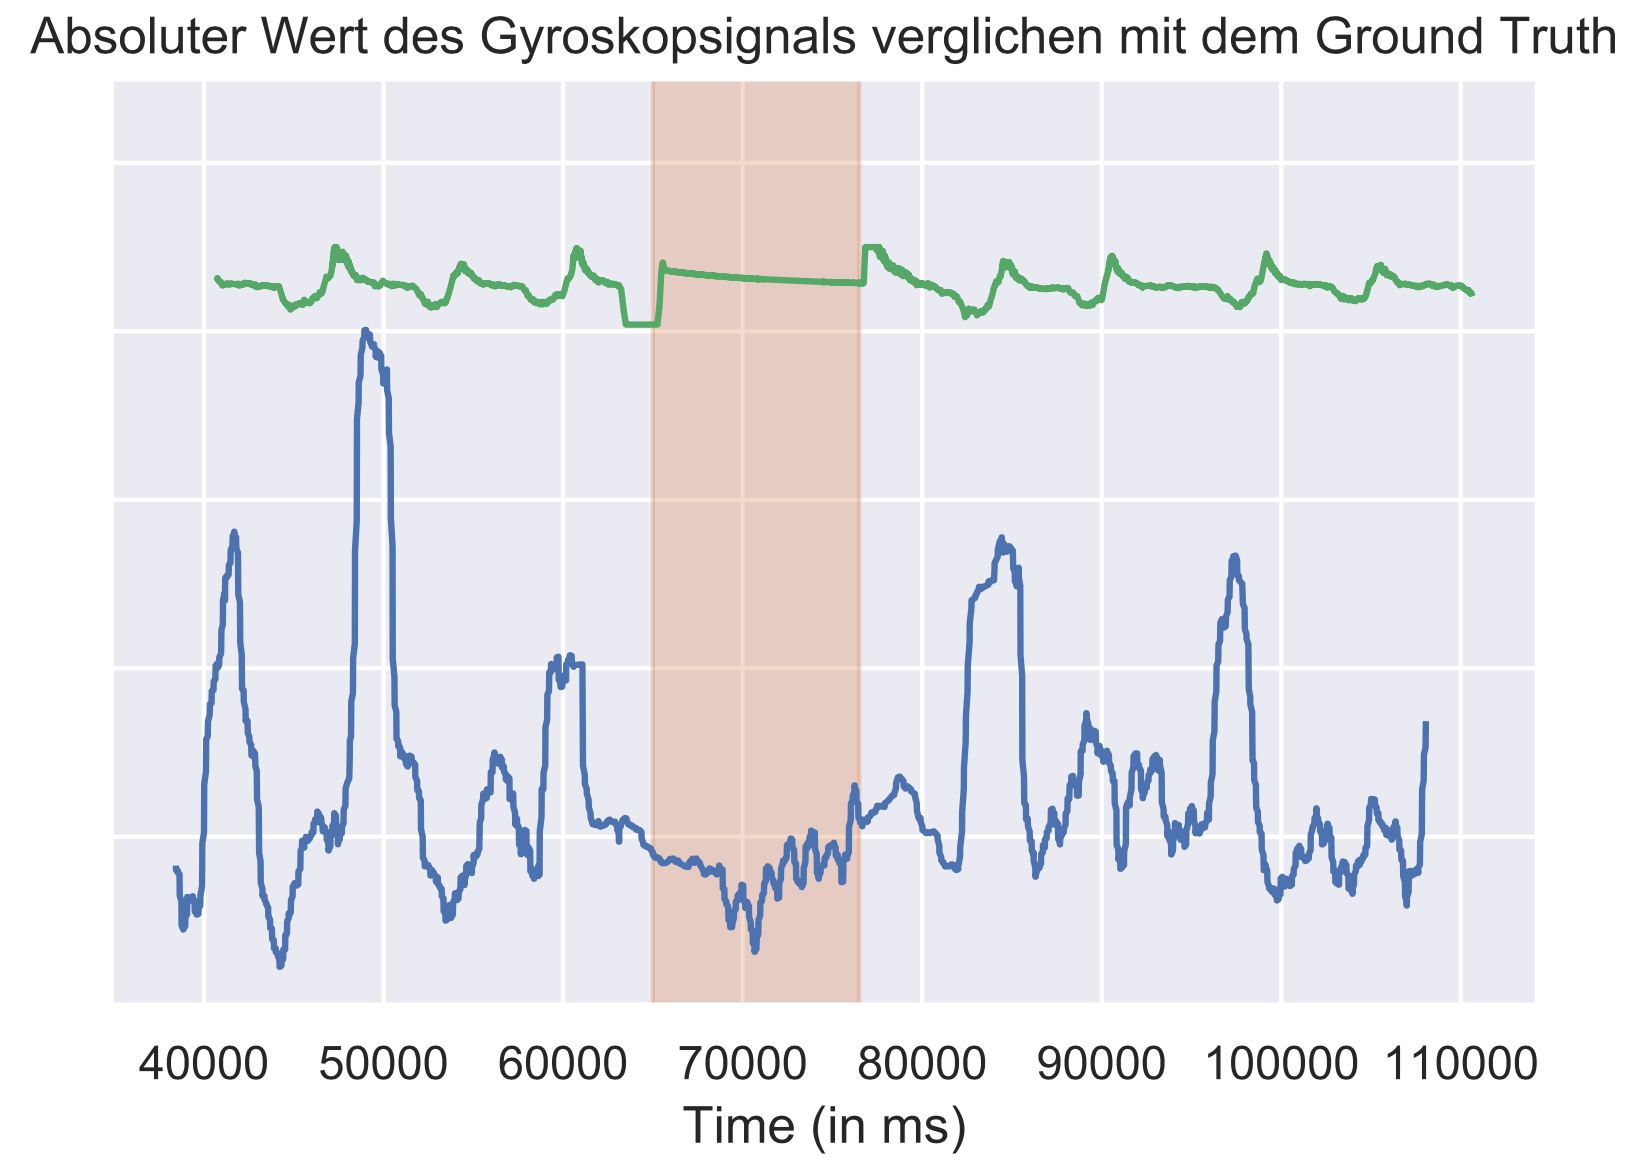
\includegraphics[width=1\textwidth]{data_analyzation/compare_raw_signal_with_flowDr_2.png}
    \end{subfigure}
  \caption{Darstellung des Signals eines Probanden während einer Messung. Zu sehen ist das Signal des Drucksensors vom PSG-Gerät, befestigt an der Nase des Probanden in grün. Zudem ist der absolute Wert, berechnet aus allen 3 Achsen des Gyroskopsignals in blau und das Apnoeereignis in orange zu sehen. Circa zwischen Sekunde 65 und 75 wurde ein Apnoeereignis simuliert. Es ist deutlich zu sehen, dass ein Apnoeereignis auch anhand der IMU-Werte zu erkennen ist. Die Berechnung des absoluten Werts ist $\sqrt{x^2+y^2+z^2}$. Beide Signale wurden normalisiert und so in der y-Achse verschoben, sodass sie vergleichbar sind.}
  \label{evaluation:rawPlot}
\end{figure}

\section{Ablauf der Evaluierung}
Im Kapitel \ref{ch:Implementierung:classification_pipeline} wurde beschrieben, wie die Features berechnet und persistiert wurden. 
Nun sind pro Studienteilnehmer für alle 3 Positionen Features berechnet worden. 
Es sind jeweils die Features für ein Fenster von 5 Sekunden und 10 Sekunden berechnet worden.
Zur Erinnerung: Jede Messung wurde in Fenster der Länge von 5, bzw. 10 Sekunden aufgeteilt, wobei jedes Fenster um eine Sekunde verschoben ist.

\subsection{Data Labeling}
Bei Supervised Learning mit Klassifikation müssen die Daten bereits markiert sein, um eine Entscheidung treffen zu können. 
Beim Abspeichern der eSense Daten ist dies bereits geschehen.
Da die Messung genau vorgibt, wann eine Person die Luft anhalten soll, beziehungsweise nicht, wird diese Information mit einem \textit{Boolean} als zusätzliches Attribut vermerkt.
Da bei der Klassifikation Features anhand der eSense Daten berechnet werden, darf dieses Attribut nicht Teil der Featureberechnung sein.
Bei einem 5 Sekunden Intervall werden circa 250 Einträge, bei einem 10 Sekunden Intervall circa 500 Einträge in eine Featureberechnung zusammenfließen, weshalb eine Markierung dieses Fensters gewählt werden muss.
Ab 50\% der markierten Einträge wird das ganze Intervall als markiert gesetzt.
Dies ist eine essenzielle Entscheidung, da beim Training des Modells nun anhand dieser Markierung entschieden wird, ob ein Intervall einen Atemaussetzer repräsentiert, oder nicht.
Mit einer Grenze von 50\% wurde eine gleichwertige Aufteilung gewählt.
Nun können die Resultate mit den Klassifikatoren verglichen werden.

\subsection{Kreuzvalidierungsverfahren}
\subsubsection{Within Subject (\textit{k-fold cross validation})}
Das erste Kreuzvalidierungsverfahren ist die \textit{K-fold cross validation}.
Bei diesem Verfahren werden alle Daten in $k$ Partitionen aufgeteilt.
Eine Partition wird als Testdatensatz und $k-1$ Partitionen werden als Trainingsdatensatz gewählt \cite{neumannMaschineLearningKIT2020}.
Somit werden alle Personen zu einem Datensatz zusammengefasst und mit der Methode \texttt{test\_train\_split} in Trainingsdaten und Testdaten aufgeteilt.
Hier wird eine Aufteilung von 70\% für die Trainingsdaten und 30\% für die Testdaten gewählt. 
Daraus ergibt sich ein \textit{score}, welcher die mittlere Genauigkeit (\textit{mean accuracy}) auf den gegebenen Testdaten, welche 30\% des Datensatzes sind, angibt.
Die Resultate sind in Abbildung \ref{evaluation:within_subject_results} zu sehen.

\begin{table}[H]
  \begin{tabular}{cc}
    \begin{minipage}{1\textwidth}
      \begin{center}
          \begin{tabular}{ | l | c | c | c | c | c | }
            \hline
            \textbf{Verfahren} & \textbf{Positionen} & \textbf{Score} & \textbf{Score} & \textbf{Score} & \textbf{Score} \\ 
            & & \textbf{$w=5\si{\s}$} & \textbf{$w=5\si{\s}$} & \textbf{$w=10\si{\s}$} & \textbf{$w=10\si{\s}$} \\
            & & \textbf{$d=1\si{\s}$} & \textbf{$d=5\si{\s}$} & \textbf{$d=1\si{\s}$} & \textbf{$d=10\si{\s}$} \\ \hline
            Random Forest & Alle &  0.87 & 0.74 & 0.89 & 0.71 \\ 
             & Rücken & 0.85 & 0.67 & 0.93 & 0.57 \\
             & Seite  & 0.86 & 0.72 & 0.89 & 0.75 \\
             & Bauch  & 0.90 & 0.85 & 0.92 & 0.66 \\ \hline
            XG Boost  & Alle & 0.88 & 0.70 & 0.92 & 0.76 \\ 
             & Rücken & 0.89 & 0.67 & 0.95 & 0.62 \\
             & Seite  & 0.90 & 0.78 & 0.92 & 0.48 \\
             & Bauch  & 0.90 & 0.75 & 0.95 & 0.63 \\ \hline
            SVM & Alle& 0.54 & 0.48 & 0.65 & 0.42 \\ 
             & Rücken & 0.60 & 0.67 & 0.72 & 0.46 \\
             & Seite  & 0.57 & 0.38 & 0.63 & 0.5 \\
             & Bauch  & 0.61 & 0.41 & 0.67 & 0.4 \\
            \hline
          \end{tabular}
      \end{center}
    \end{minipage}
  \end{tabular}

  \caption{Ergebnisse des Kreuzvalidierungsverfahrens innerhalb eines Subjects mit einer Aufteilung von 70\% Trainings- und 30\% Testdaten. Alle Personen der Nutzerstudie wurden verwendet. $w$ steht für die Fenstergröße, $d$ für die Verschiebung der aneinanderfolgenden Fenster.}
  \label{evaluation:within_subject_results}
\end{table}

Die Tabelle zeigt die Ergebnisse verschiedener Klassifikationsalgorithmen mit verschiedenen Datensätzen.
Pro Klassifikationsalgorithmus wurden alle Positionen, sowie jede Position einzeln betrachtet, d.h jede Position jeder Person.
Jede Kombination aus Klassifikationsalgorithmus und gewähltem Datensatz wurde nun mit den Fenstergrößen von $5\si{\s}$ und $10\si{\s}$ mit einer Verschiebung von $1\si{\s}$ und einer Verschiebung der Fenstergröße evaluiert.
Somit wurden die Fenstergrößen mit und ohne überlappende Fenster getestet.
Die Resultate zeigen, dass der \textit{score} mit überlappenden Fenstern deutlich höher ist.
Dies könnte daran liegen, dass deutlich mehr Fenster pro Datensatz existieren, falls eine Überlappung der aneinanderfolgenden Fenster stattfindet.
Jedoch ist es auch möglich, dass Teile der überlappenden Fenster bereits erkannt und markiert wurden.
Dadurch ist der überlappende Teil eventuell in den Trainingsdaten vorhanden und eine Klassifizierung ist einfach für den Klassifikationsalgorithmus.

\subsubsection{Leave One Subject Out (LOSO)}
Neben dem k-fachen Kreuzvalidierungsverfahren wird das das \textit{Leave One Subject Out} (\textit{LOSO}) Kreuzvalidierungsverfahren hinzugezogen. 
Hierbei wird ein Modell anhand der Daten der Studienteilnehmer trainiert, jedoch wird ein Datensatz eines Studienteilnehmers ausgelassen. 
Dieser eine Datensatz wird schließlich verwendet, um eine Vorhersage anhand der Trainingsdaten zu treffen, ohne durch interne Trainingsdaten optimiert sein zu können.
Im Folgenden wurde das LOSO Kreuzvalidierungsverfahren mit den beiden Klassifikationsalgorithmen \textit{Random Forest} und \textit{XGBoost} durchgeführt. 
Es wurde jede Person einmal ausgelassen und auf den Trainingsdatensatz angewandt, welcher diese Person nicht enthält. 
Somit entstehen 7 Resultate, von denen nun der Mittelwert gebildet wird.
Die Resultate sind in den Abbildungen \ref{evaluation:random_forest_loso:person6} und \ref{evaluation:xgboost_loso:person6} beispielhaft an Person 6 dargestellt.
Im Anhang sind weitere Abbildungen anderer Personen zu finden.
Die Abbildungen listen die Häufigkeit der Vorhersagen für jede einzelne Sekunde auf. 
Da eine Sekunde aufgrund der überlappenden Fenster in mehreren Fenstern vorkommt, summieren sich die Vorhersagen pro Sekunde maximal auf die Fenstergröße.
Zu Erkennen ist, dass die Fenstergröße von $10\si{\s}$ deutlich bessere Ergebnisse liefert, als eine Fenstergröße von $5\si{\s}$. 
XGBoost neigt bei einer Fenstergröße von $5\si{\s}$ zum Overfitting, ebenso wie Random Forest. 
Der Mittelwert aller Ergebnisse des LOSO Kreuzvalidierungsverfahrens sind im \textit{Precision} und \textit{Recall} der unterliegenden Tabelle der Beispiele bei Person 6 mit dem Mittelwert zusammengetragen worden. 
Zu sehen ist, dass XGBoost bessere Ergebnisse liefert als Random Forest.
% \todo{schreibe darüber, was die ergebnisse von LOSO aussagen} \newline
Des weiteren, um mögliche Positionsabhängigkeiten zu erkennen, wurde dasselbe erneut evaluiert, jedoch nur mit den einzelnen Positionsdaten der jeweiligen Person. 
In der Tabelle \ref{evaluation:loso_classification_results} sind die Resultate zu sehen.
%\todo{schreibe darüber, was die ergebnisse der einzelnen personen aussagen}

\subsection{Relevante Features}
Jede Klassifikation ergab ein Resultat, welches durch einzelne Features entschieden wurde. 
Das Python-Framework \texttt{scikit-learn} beinhaltet \texttt{feature\_importances\_} und zeigt die Relevanz der einzelnen Features in einem Plot.
Um einen kleinen Überblick zu bekommen, welche Features entscheidend für die Evaluation waren, sind nun einige aufgelistet.
\begin{itemize}
    \item \texttt{gyroZ partial autocorrelation}
    \item \texttt{gytoX fft coefficient}
    \item \texttt{gyroX agg autocorrelation}
    \item \texttt{accY autocorrelation}
    \item \texttt{gyroY change quantiles }
    \item \texttt{gyroZ fft coefficient}
\end{itemize}
Diese Features wurden mittels \texttt{tsfresh} berechnet und waren bei der Klassifikation des Kreuzvalidierungsverfahrens entscheidened \cite{TsfreshTsfresh12}.
Die partielle Autokorrelationfunktion (\texttt{partial autocorrelation}) beschreibt die Abhänigkeit zwischen den Werten der Zeitreihen. 
Zudem wird ein zeitlicher linearer Zusammenhang der verschiedenen Werte gemessen.
Somit haben sich die Werte in diesem Fenster zwischen den Werten weniger verändert und ähneln somit eher den positiv markierten Trainingsdaten.

Die \textit{Schnelle Fourier-Transformation} berechnet effizient die diskrete Fourier-Transformation.
Damit können zeitdiskrete Signale in Frequenzanteile zerlegt werden. 
Es wird aus einer Darstellung, bestehend aus einem Zeit- und Abtastwert in einer Darstellung, bestehend aus einem Frequenzanteil, einer Amplitude und einer Phase überführt.
Die Funktion \texttt{fft\_coefficient} in \texttt{tsfresh} berechnet die Fourier Koeffizienten einer eindimensionalen diskreten Fouriertransformation für eine reale Eingabe mit dem Algorithmus der Fast-Fourier-Transformation:
\[A_k = \sum_{m=0}^{n-1} a_m \exp ^ {-2\pi i \frac{mk}{n}}, \hspace{1cm} k = 0,\dots,n-1\]
Die bei der Apnoephase geringe Amplitude ist hier erkennbar und detektierbar, womit eine Klassifikation ermöglicht wird.
Die Aggregation \texttt{agg\_autocorrelation} berechnet den Wert der Autokorrelationsfunktion $f_{agg}$ (beispielsweise die Varianz oder den Mittelwert) über die Autokorrelation $R(l)$ für die verschiedenen Fenster. 
\[R(l) = \frac{1}{(n-l)\sigma ^2} \sum_{t=1}^{n-l} (X_t - \mu) (X_{t+l} - \mu)\]
$X_i$ sind hierbei  die Werte der Timeseries, $n$ deren Länge. 
$\sigma$ und $\mu$ sind Schätzwerte für die Varianz und den Mittelwert.

Ein weiteres Feature, welches ausschlaggebend für die Klassifikation ist, ist der Wechsel der Quantilwerte (\texttt{change\_quantiles}).
Pro Fenster wird ein $ql$ niedriges Quantil und ein $qh$ hohes Quantil berechnet. 
Anschließend wird der durchschnittliche, absolute Wert der aufeinanderfolgenden Änderungen der Reihe x innerhalb dieser Quantile berechnet.
Dadurch werden starke Veränderungen deutlich und stellen klar, dass in diesem Fenster kein Apnoe stattfindet. 


%%%%%%%%%%%%%%%%%%%        RANDOM FOREST 5 sec %%%%%%%%%%%%%%%%%%%%%%%%%%%%%%%%%
\begin{figure}[H]
  \textbf{Random Forest ($w=5\si{\s}$, $d=1\si{\s}$)}
    \centering
    \begin{subfigure}{1\textwidth}
        \includegraphics[width=1\textwidth]{evaluation/loso_5sec/random_forest_loso/Random Forest (Leave one Subject out: Person 6 back).png}
        %\caption{Resultate der Person 6 auf dem Rücken liegend.}
      \end{subfigure}
      \begin{subfigure}{1\textwidth}
        \includegraphics[width=1\textwidth]{evaluation/loso_5sec/random_forest_loso/Random Forest (Leave one Subject out: Person 6 side).png}
        %\caption{Resultate der Person 6 auf der Seite liegend.}
      \end{subfigure}
      \begin{subfigure}{1\textwidth}
        \includegraphics[width=1\textwidth]{evaluation/loso_5sec/random_forest_loso/Random Forest (Leave one Subject out: Person 6 stomach).png}
        %\caption{Resultate der Person 6 auf dem Bauch liegend.}
    \end{subfigure}
    \begin{subfigure}{1\textwidth}
        \begin{center}
            \begin{tabular}{ | l | c | c | r | }
              \hline
               & precision & recall & f1-score\\ \hline
              0 & 0.92 & 0.75 & 0.81 \\ \hline
              1 & 0.75 & 0.67 & 0.47 \\
              \hline
            \end{tabular}
        \end{center}
        \caption{Random Forest mit dem Kreuzvalidierungsverfahren: Die Tabelle zeigt den Mittelwert aller Vorhersagen der einzelnen Personen.}
        \label{implementation:app:screenshots:user_studies_information}
    \end{subfigure}
    \newline
    \vspace*{1 cm}
    \newline
    \textbf{Random Forest ($w=10\si{\s}$, $d=1\si{\s}$)}
    \begin{subfigure}{1\textwidth}
      \includegraphics[width=1\textwidth]{evaluation/loso_10sec/random_forest_loso/Random Forest (Leave one Subject out: Person 6 back).png}
      %\caption{Resultate der Person 6 auf dem Rücken liegend.}
    \end{subfigure}
    \begin{subfigure}{1\textwidth}
      \includegraphics[width=1\textwidth]{evaluation/loso_10sec/random_forest_loso/Random Forest (Leave one Subject out: Person 6 side).png}
      %\caption{Resultate der Person 6 auf der Seite liegend.}
    \end{subfigure}
    \begin{subfigure}{1\textwidth}
      \includegraphics[width=1\textwidth]{evaluation/loso_10sec/random_forest_loso/Random Forest (Leave one Subject out: Person 6 stomach).png}
      %\caption{Resultate der Person 6 auf dem Bauch liegend.}
  \end{subfigure}

  \begin{subfigure}{1\textwidth}
      \begin{center}
          \begin{tabular}{ | l | c | c | r | }
            \hline
             & precision & recall & f1-score\\ \hline
            0 & 0.92 & 0.77 & 0.83\\ \hline
            1 & 0.77 & 0.67 & 0.5\\
            \hline
          \end{tabular}
      \end{center}
      \caption{Random Forest mit dem Kreuzvalidierungsverfahren (LOSO): Die Tabelle zeigt den Mittelwert aller Vorhersagen der einzelnen Personen.}
      \label{implementation:app:screenshots:user_studies_information}
  \end{subfigure}
    \caption{Das Kreuzvalidierungsverfahren (LOSO) mit dem Klassifikationsalgorithmus Random Forest. Das Modell wurde auf allen Personen, exklusive einer Person trainiert. Auf alle Positionen dieser einen Person wurde eine Vorhersage getroffen. Am Beispiel hier sind die Resultate von Person 6 zu sehen. Die blauen Bereiche sind die, in denen die Luft angehalten wurde, die orange Kurve zeigt die Vorhersage ($w=$ Fenstergröße, $d=$ Verschiebung der Fenster).}
\label{evaluation:random_forest_loso:person6}
\end{figure}

%%%%%%%%%%%%%%%%%%%        XG BOOST 5 sec %%%%%%%%%%%%%%%%%%%%%%%%%%%%%%%%%

\begin{figure}[H]
  \textbf{XG Boost ($w=5\si{\s}$, $d=1\si{\s}$)}
    \centering
    \begin{subfigure}{1\textwidth}
        \includegraphics[width=1\textwidth]{evaluation/loso_5sec/xg_boost_loso/XG Boost (Leave one Subject out: Person 6 back).png}
        %\caption{Resultate der Person 6 auf dem Rücken liegend.}
      \end{subfigure}
      \begin{subfigure}{1\textwidth}
        \includegraphics[width=1\textwidth]{evaluation/loso_5sec/xg_boost_loso/XG Boost (Leave one Subject out: Person 6 side).png}
        %\caption{Resultate der Person 6 auf der Seite liegend.}
      \end{subfigure}
      \begin{subfigure}{1\textwidth}
        \includegraphics[width=1\textwidth]{evaluation/loso_5sec/xg_boost_loso/XG Boost (Leave one Subject out: Person 6 stomach).png}
        %\caption{Resultate der Person 6 auf dem Bauch liegend.}
    \end{subfigure}

    \begin{subfigure}{1\textwidth}
        \begin{center}
            \begin{tabular}{ | l | c | c | r | }
              \hline
               & precision & recall & f1-score \\ \hline
              0 & 0.93 & 0.71 & 0.79 \\ \hline
              1 & 0.72 & 0.69 & 0.47 \\
              \hline
            \end{tabular}
        \end{center}
        \caption{XGBoost mit dem Kreuzvalidierungsverfahren (LOSO): Die Tabelle zeigt den Mittelwert aller Vorhersagen der einzelnen Personen.}
        \label{implementation:app:screenshots:user_studies_information}
    \end{subfigure}
    \newline
    \vspace*{1 cm}
    \newline
    \textbf{XG Boost ($w=10\si{\s}$, $d=1\si{\s}$)}
    \begin{subfigure}{1\textwidth}
      \includegraphics[width=1\textwidth]{evaluation/loso_10sec/xg_boost_loso/XG Boost (Leave one Subject out: Person 6 back).png}
      %\caption{Klassifikationsresultate der Person 6. Die Messung wurde auf dem Rücken liegend durchgeführt.}
    \end{subfigure}
    \begin{subfigure}{1\textwidth}
      \includegraphics[width=1\textwidth]{evaluation/loso_10sec/xg_boost_loso/XG Boost (Leave one Subject out: Person 6 side).png}
      %\caption{Klassifikationsresultate der Person 6. Die Messung wurde auf der Seite liegend durchgeführt.}
    \end{subfigure}
    \begin{subfigure}{1\textwidth}
      \includegraphics[width=1\textwidth]{evaluation/loso_10sec/xg_boost_loso/XG Boost (Leave one Subject out: Person 6 stomach).png}
      %\caption{Klassifikationsresultate der Person 6. Die Messung wurde auf dem Bauch liegend durchgeführt.}
  \end{subfigure}

  \begin{subfigure}{1\textwidth}
      \begin{center}
          \begin{tabular}{ | l | c | c | r | }
            \hline
             & precision & recall & f1-score \\ \hline
            0 & 0.93 & 0.74 & 0.8 \\ \hline
            1 & 0.74 & 0.75 & 0.5 \\
            \hline
          \end{tabular}
      \end{center}
      \caption{XGBoost mit dem Kreuzvalidierungsverfahren (LOSO): Die Tabelle zeigt den Mittelwert aller Vorhersagen der einzelnen Personen.}
      \label{implementation:app:screenshots:user_studies_information}
  \end{subfigure}
    \caption{Das Kreuzvalidierungsverfahren (LOSO) mit dem Klassifikationsalgorithmus XG Boost: Das Modell wurde auf allen Personen, exklusive einer Person trainiert. Auf alle Positionen dieser einen Person wurde eine Vorhersage getroffen. Am Beispiel hier sind die Resultate von Person 6 zu sehen. Die blauen Bereiche sind die, in denen die Luft angehalten wurde, die orange Kurve zeigt die Vorhersage ($w=$ Fenstergröße, $d=$ Verschiebung der Fenster).}
\label{evaluation:xgboost_loso:person6}
\end{figure}

%%%%%%%%%%%%%%%%%%%        Position based results  5 sec %%%%%%%%%%%%%%%%%%%%%%%%%%%%%%%%%
\begin{table}
  \begin{tabular} {cc}
    \begin{minipage}{1\linewidth}
      \begin{center}
          \begin{tabular}{ | l | c | c | c | c | c | r | }
            \hline
            Klassifikation & Fenstergröße & Position & & precision & recall & f1-score \\ \hline
            Random Forest & 5s & Seite & 0 & 0.86 & 0.76 & 0.81 \\ 
                          &    &       & 1 & 0.76 & 0.57 & 0.48 \\ \hline
                          &    & Rücken& 0 & 0.90 & 0.79 & 0.83 \\ 
                          &    &       & 1 & 0.83 & 0.52 & 0.39 \\ \hline
                          &    & Bauch & 0 & 0.92 & 0.72 & 0.70 \\ 
                          &    &       & 1 & 0.72 & 0.69 & 0.52 \\ \hline
            \hline
            XG Boost & 5s & Seite & 0 & 0.91 & 0.67 & 0.71 \\
                     &    &       & 1 & 0.67 & 0.61 & 0.35 \\ \hline
                     &    & Rücken& 0 & 0.90 & 0.74 & 0.80 \\ 
                     &    &       & 1 & 0.75 & 0.57 & 0.38 \\ \hline
                     &    & Bauch & 0 & 0.94 & 0.71 & 0.74 \\ 
                     &    &       & 1 & 0.71 & 0.72 & 0.55 \\ \hline
            \hline
            Random Forest & 10s & Seite & 0 & 0.89 & 0.77 & 0.83 \\ 
                          &     &       & 1 & 0.80 & 0.67 & 0.5 \\ \hline
                          &     & Rücken& 0 & 0.89 & 0.83 & 0.85 \\
                          &     &       & 1 & 0.82 & 0.52 & 0.41 \\ \hline
                          &     & Bauch & 0 & 0.93 & 0.71 & 0.74 \\
                          &     &       & 1 & 0.71 & 0.70 & 0.49 \\ \hline
            \hline
            XGBoost & 10s & Seite & 0 & 0.90 & 0.78 & 0.78 \\
                    &     &       & 1 & 0.78 & 0.71 & 0.47 \\ \hline
                    &     & Rücken& 0 & 0.90 & 0.85 & 0.86 \\
                    &     &       & 1 & 0.85 & 0.50 & 0.44 \\ \hline
                    &     & Bauch & 0 & 0.94 & 0.72 & 0.75 \\
                    &     &       & 1 & 0.72 & 0.70 & 0.53 \\ \hline
          \end{tabular}
          \smallskip
          \\ Random Forest (only side, \textit{window: 5s})
      \end{center}
      %\label{evaluation:5s:random_forest_loso_side}
  \end{minipage} 
    
  \end{tabular}
  \caption{Zu sehen sind die Klassifikationsergebnisse mit dem Kreuzvalidierungsverfahren bei einer Fenstergröße von 5, bzw. 10 Sekunden, welche um 1 Sekunde verschoben wurden. Es wurde immer eine Person aus dem Trainieren des Modells ausgelassen. Auf diese Person wurde anschließend eine Vorhersage getroffen. Jede Person wurde einmel in dem Modell außen vorgelassen und auf dieses Modell vorhergesagt. Das zu sehende Resultat ist der Mittelwert aller Resultate des Kreuzvalidierungsverfahrens der einzelnen Positionen der Position.}
  \label{evaluation:loso_classification_results}  
\end{table}

  % \todo{ich habe gelernt}
% \begin{itemize}
%     \item auswertungsdaten: Auf dem rücken liegende ddaten sind am vielversprechendsten
%     \item die atempausen können einigermaßen klassifiziert werden
%     \item rauschen entfernen bringt nix vermutlich wegen tsfresh, da es das schon macht, also es kommen
%     \item 10 sekunden window size ist besser als 5 sekunden window size
%     \item xgboost bringt bessere resultate, als random forest und svm, braucht aber auch länger
% \end{itemize}

% gibt earables, die blutsauerstoff und puls mittracken können
% plus grafik telegram tobi